
\documentclass[11pt]{article}

\usepackage{amsmath, amssymb, amsfonts}
\usepackage{graphicx}
\graphicspath{{figures/}}
\usepackage{hyperref}
\usepackage{array}
\usepackage{geometry}
\usepackage{booktabs}
\usepackage{multirow}
\usepackage{tikz}
\usepackage{pgfplots}
\usepackage{float}

\usetikzlibrary{positioning, arrows.meta, shapes.geometric}
\pgfplotsset{compat=1.18}

\geometry{
 a4paper,
 total={170mm,257mm},
 left=20mm,
 top=20mm,
}

\hypersetup{
 colorlinks=true,
 linkcolor=blue,
 urlcolor=blue
}

\title{\textbf{MNIST Handwritten Digit Classification:\\
A Comparison of Single-Layer, Multi-Layer and Convolutional Neural Networks}}

\author{}
\date{}

\begin{document}

\maketitle

\begin{abstract}
This report studies a simple but important machine learning task: recognizing handwritten digits from images. Each image in the MNIST dataset contains one digit from 0 to 9, and the model must predict the correct label. Three models were trained and compared in Kaggle notebooks: a single-layer perceptron, a multilayer perceptron (MLP), and a convolutional neural network (CNN) based on LeNet.

The report explains the problem in easy language, describes how each model works, and compares the models using validation results, confusion matrices, learned features, and Kaggle submission scores. The main result is clear. The perceptron works as a simple baseline, the MLP performs much better because it can learn nonlinear patterns, and the CNN gives the best overall performance because it can use the 2D structure of the image directly. This makes the CNN the most suitable model for handwritten digit recognition in this assignment.
\end{abstract}

\section{Kaggle Implementation}

All final experiments for this assignment were run in Kaggle notebooks. This was useful because the competition data is already available on Kaggle, the notebook environment makes the training process easy to reproduce, and the generated CSV files can be submitted directly to the \emph{Digit Recognizer} competition.

To satisfy the assignment requirement of making separate entries for each classifier, the work was split into three public Kaggle notebooks:
\begin{itemize}
    \item \href{https://www.kaggle.com/code/zaeemnasir7/perceptron-mnist}{Perceptron MNIST notebook}
    \item \href{https://www.kaggle.com/code/zaeemnasir7/mlp-mnist}{MLP MNIST notebook}
    \item \href{https://www.kaggle.com/code/zaeemnasir7/cnn-lenet-mnist}{CNN (LeNet) MNIST notebook}
\end{itemize}

Each notebook trains one model only and creates one submission file:
\begin{itemize}
    \item perceptron $\rightarrow$ \texttt{submission\_\allowbreak perceptron.csv}
    \item MLP $\rightarrow$ \texttt{submission\_\allowbreak mlp.csv}
    \item CNN $\rightarrow$ \texttt{submission\_\allowbreak cnn.csv}
\end{itemize}

This makes the comparison very clear because each model has its own code, its own training results, and its own Kaggle leaderboard score.

\section{Introduction}

Classification means assigning the correct label to an input. In this assignment, the input is a small grayscale image of a handwritten digit, and the correct label is one of the numbers 0 to 9. The task sounds simple, but it becomes challenging because different people write the same digit in different ways.

This report compares three neural network models that solve the same problem in different ways: a perceptron, a multilayer perceptron (MLP), and a convolutional neural network (CNN) based on LeNet. The aim is not only to get good accuracy, but also to understand why some models perform better than others.

\subsection{Project Overview in Simple Words}

The whole project can be understood in four simple steps:
\begin{enumerate}
    \item take an image of a handwritten digit,
    \item train a model to predict which digit it is,
    \item test the model on unseen images,
    \item submit the predictions to Kaggle and compare the scores.
\end{enumerate}

The three models used in this report are summarized in Table~\ref{tab:plaincompare}. The idea is to start from the simplest model and then move to models that can learn richer image patterns.

\begin{table}[H]
\centering
\begin{tabular}{>{\raggedright\arraybackslash}p{2.4cm} >{\raggedright\arraybackslash}p{6.0cm} >{\raggedright\arraybackslash}p{4.1cm}}
\toprule
\textbf{Model} & \textbf{Simple idea} & \textbf{Main strength} \\
\midrule
Perceptron & One linear layer looks at all 784 pixels at once and directly predicts the class. & Fast and easy baseline. \\
MLP & Several fully connected layers learn nonlinear combinations of pixel patterns. & Learns more complex decision boundaries. \\
CNN (LeNet) & Convolution and pooling layers learn small image patterns such as edges and strokes. & Best match for image data. \\
\bottomrule
\end{tabular}
\caption{A very simple summary of the three models used in this report.}
\label{tab:plaincompare}
\end{table}

\section{Real-World Meaning of Classification}

Classification appears in many real-world applications. The underlying idea is always the same: an input sample is mapped to a discrete category. The nature of the input, however, can vary widely from one application domain to another.

\begin{figure}[H]
\centering
\resizebox{0.98\textwidth}{!}{%
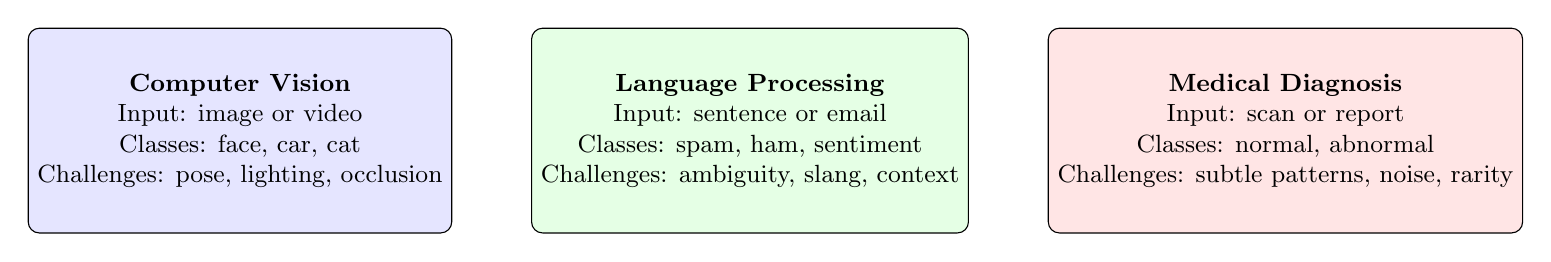
\begin{tikzpicture}[node distance=10mm and 10mm, every node/.style={font=\small}]
\node[draw, rounded corners, fill=blue!10, minimum width=4.3cm, minimum height=2.6cm, align=center] (cv) {\textbf{Computer Vision}\\Input: image or video\\Classes: face, car, cat\\Challenges: pose, lighting, occlusion};
\node[draw, rounded corners, fill=green!10, minimum width=4.3cm, minimum height=2.6cm, align=center, right=of cv] (nlp) {\textbf{Language Processing}\\Input: sentence or email\\Classes: spam, ham, sentiment\\Challenges: ambiguity, slang, context};
\node[draw, rounded corners, fill=red!10, minimum width=4.3cm, minimum height=2.6cm, align=center, right=of nlp] (med) {\textbf{Medical Diagnosis}\\Input: scan or report\\Classes: normal, abnormal\\Challenges: subtle patterns, noise, rarity};
\end{tikzpicture}%
}
\caption{Examples of classification problems in different real-world domains.}
\label{fig:domains}
\end{figure}

In \textbf{computer vision}, classification systems may identify objects in photographs, distinguish traffic signs for autonomous driving, or recognize faces for attendance systems. In \textbf{natural language processing}, classification is used for spam detection, sentiment analysis, intent recognition in chatbots, and topic labeling of documents. In the \textbf{medical domain}, classification is used to identify disease categories from X-rays, MRI scans, pathology images, or even patient records.

These examples show why classification is so important. It provides a way to convert raw data into meaningful decisions. However, these decisions are difficult because the same class can appear in many different forms. A cat may look different in each photo, a positive movie review may use many different expressions, and a disease may appear differently across patients. The same challenge appears in handwritten digit recognition: every person writes the same digit in a slightly different way.

\section{Challenges in Automatic Classification}

Writing programs to classify objects automatically has always been difficult because real data is highly variable. A simple rule-based system works only when the appearance of each class is very consistent. In practice, this is rarely true.

Handwritten digit recognition is a good example. The digit ``2'' written by one person may look very different from the digit ``2'' written by another. Some writers use curved strokes, others use sharp corners. The digit ``1'' may look similar to a handwritten ``7'', and ``4'' may resemble ``9'' in some styles. Even the same person may write the same digit differently at different times.

Several factors make automatic classification challenging:
\begin{itemize}
    \item \textbf{Intra-class variation:} samples from the same class can look different from one another.
    \item \textbf{Inter-class similarity:} samples from different classes can sometimes look very similar.
    \item \textbf{Noise and distortion:} images may contain blur, background noise, weak strokes, or small shifts.
    \item \textbf{High dimensionality:} a $28 \times 28$ image contains 784 pixel values, so even a small image has many features.
    \item \textbf{Lack of explicit rules:} it is difficult to manually write a complete set of rules that correctly handles all possible handwriting styles.
\end{itemize}

These difficulties explain why data-driven learning is necessary. Instead of trying to manually define every possible writing pattern, machine learning models learn directly from labeled examples. The training process adjusts the model parameters so that the model gradually becomes better at separating one class from another.

\section{MNIST Dataset}

The MNIST dataset is one of the most widely used benchmark datasets in machine learning and deep learning. It contains grayscale images of handwritten digits from 0 to 9. Each image has size $28 \times 28$ pixels, which means every sample contains 784 intensity values.

The dataset contains:
\begin{itemize}
    \item 60,000 training images,
    \item 10,000 test images,
    \item 10 output classes corresponding to the digits 0 through 9.
\end{itemize}

MNIST is a good benchmark dataset for several reasons. First, it is small enough to allow fast experimentation, which is useful for beginners and for model comparison. Second, it is large enough to reveal meaningful differences between models. Third, it is clean and standardized, which makes it possible to compare results across different studies and implementations.

Handwritten digit recognition is more challenging than recognizing typed characters because typed characters usually follow a fixed font and consistent stroke pattern. Handwritten digits, in contrast, vary in thickness, orientation, size, style, and shape. This makes MNIST simple enough to learn from, but still difficult enough to highlight important differences between models.

\begin{figure}[H]
\centering
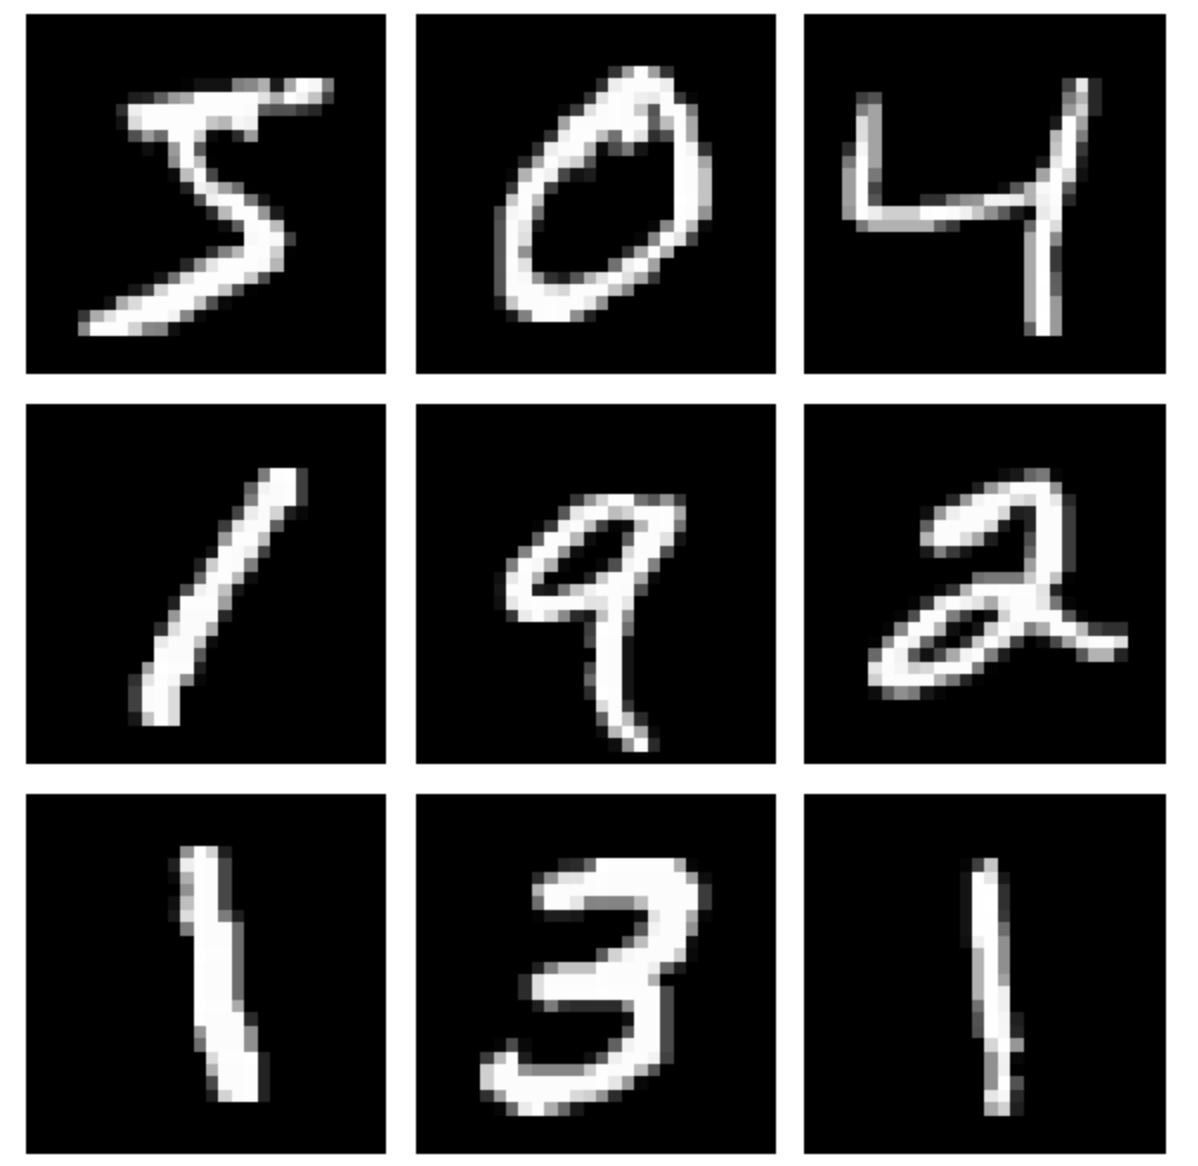
\includegraphics[width=0.70\textwidth]{mnist_samples.png}
\caption{Examples of handwritten digits from the MNIST dataset.}
\label{fig:mnist_samples}
\end{figure}

\section{Single Layer Neural Network (Perceptron)}

\subsection{The Perceptron as a Linear Classifier}

The perceptron is one of the simplest neural models for classification. For an input vector $x \in \mathbb{R}^{784}$, the model computes a weighted sum of the input features and adds a bias:
\begin{equation}
z = w^T x + b
\end{equation}

For binary classification, the sign of $z$ determines on which side of the decision boundary the sample lies. The decision boundary itself is defined by:
\begin{equation}
w^T x + b = 0
\end{equation}

This equation describes a hyperplane in feature space. The weight vector $w$ has several useful interpretations:
\begin{itemize}
    \item As a \textbf{template}, it describes what pattern the model associates with a class.
    \item As a \textbf{normal vector}, it is perpendicular to the separating hyperplane.
    \item As a \textbf{feature importance vector}, it indicates how strongly each input dimension contributes to the decision.
\end{itemize}

The bias term $b$ can also be interpreted in two ways. It acts as a negative threshold that must be overcome before the model predicts a class, and geometrically it shifts the separating hyperplane away from the origin.

For MNIST, the task is not binary but ten-class classification. Therefore, the perceptron is extended to a multiclass linear model:
\begin{equation}
z = Wx + b
\end{equation}
where $W \in \mathbb{R}^{10 \times 784}$ and $b \in \mathbb{R}^{10}$. Each row of $W$ corresponds to one digit class. The output vector $z$ contains one score, or \emph{logit}, for each class.

\subsection{Supervised Learning, Softmax, and Loss Functions}

In supervised learning, training data is given as labeled pairs
\[
\{(x_i, y_i)\}_{i=1}^{N},
\]
where $x_i$ is an input image and $y_i$ is its correct class label. The goal is to learn parameters $W$ and $b$ that minimize classification error on both seen and unseen data.

To convert logits into probabilities, the softmax function is used:
\begin{equation}
\hat{y}_k = \frac{e^{z_k}}{\sum_{j=1}^{10} e^{z_j}}, \qquad k=1,\dots,10
\end{equation}

The prediction is the class with the highest probability. During training, the model is optimized using the cross-entropy loss:
\begin{equation}
L(x,y) = - \sum_{k=1}^{10} y_k \log(\hat{y}_k)
\end{equation}
where $y_k$ is the one-hot encoded target for class $k$.

The overall optimization objective is:
\begin{equation}
\min_{W,b} \; \frac{1}{N} \sum_{i=1}^{N} L(x_i, y_i)
\end{equation}

This turns learning into an optimization problem. A gradient-based optimizer repeatedly updates the parameters so as to reduce the loss:
\begin{equation}
\theta_{t+1} = \theta_t - \eta \nabla_{\theta} L
\end{equation}
where $\theta$ represents all trainable parameters and $\eta$ is the learning rate.

\subsection{Representational Limitations of a Single-Layer Model}

The strength of the perceptron is its simplicity, but that simplicity also limits what it can represent. Because the perceptron is a linear model, it can only learn linear decision boundaries. If a task requires a curved or highly irregular boundary, a single layer is not expressive enough.

This limitation is important for image classification. Handwritten digits are not separated by simple straight lines in the 784-dimensional pixel space. Different digits may overlap in some regions and require more complex decision surfaces. A well-known example is the XOR problem, which cannot be solved by a single linear separator.

The basic perceptron can still be extended to multiclass classification in different ways:
\begin{itemize}
    \item \textbf{One-vs-rest classifiers:} train one binary classifier per class.
    \item \textbf{Multiclass softmax classifier:} produce scores for all classes at once and normalize them with softmax.
\end{itemize}
In this assignment, the softmax formulation is more natural because it directly models the ten-way digit classification problem.

\subsection{Implementation Summary}

For the MNIST perceptron, each image is flattened from a $28 \times 28$ array into a 784-dimensional vector. The model contains a single linear layer with 10 outputs, one for each class. Cross-entropy loss is used for learning, and model parameters are updated with a gradient-based optimizer. This implementation is simple, fast to train, and serves as a strong baseline for comparison with deeper models.

\begin{figure}[H]
\centering
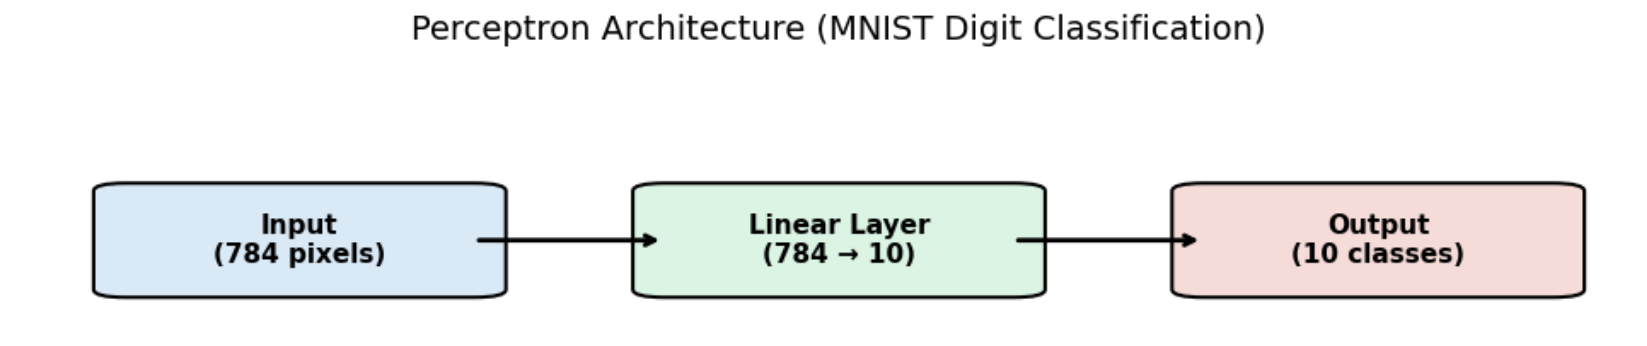
\includegraphics[width=0.85\textwidth]{perceptron_architecture.png}
\caption{Architecture of the single-layer perceptron used for MNIST classification.}
\label{fig:perceptron_arch}
\end{figure}

\begin{figure}[H]
\centering
\includegraphics[width=0.85\textwidth]{perceptron_curves.png}
\caption{Training and validation loss and accuracy curves for the perceptron model.}
\label{fig:perceptron_curves}
\end{figure}

\begin{figure}[H]
\centering
\includegraphics[width=0.75\textwidth]{perceptron_confusion.png}
\caption{Confusion matrix of the perceptron model.}
\label{fig:perceptron_confusion}
\end{figure}

\subsection{Perceptron Results and Interpretation}

The perceptron worked as a simple baseline. In the final Kaggle notebook, it achieved \textbf{91.76\%} validation accuracy, a macro F1-score of \textbf{0.9167}, and a training time of \textbf{11.90 seconds} with only \textbf{7,850} trainable parameters. This is a useful result for such a simple model, but it also shows the limitation of a linear classifier on image data.

\begin{figure}[H]
\centering
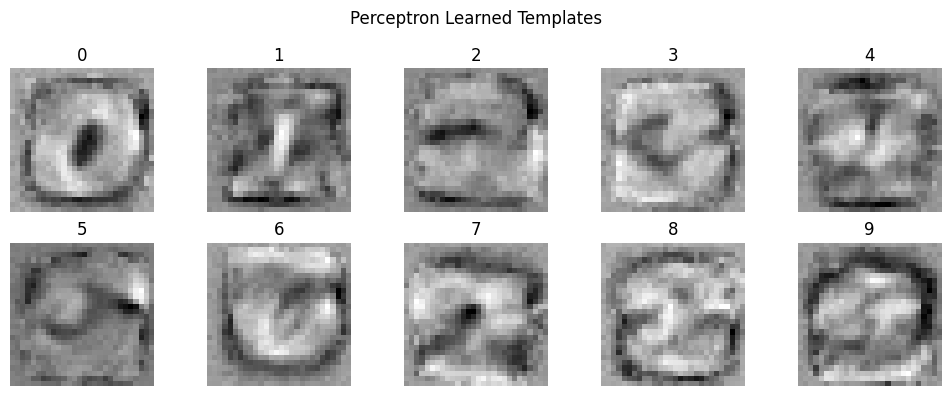
\includegraphics[width=0.72\textwidth]{perceptron_templates.png}
\caption{Learned weight templates of the perceptron model.}
\label{fig:perceptron_templates}
\end{figure}

The learned templates in Figure~\ref{fig:perceptron_templates} look like rough and blurry digit prototypes. This gives an intuitive explanation of how the perceptron works: it tries to match the input image to a simple class template. That idea is helpful, but it is still not strong enough to handle all handwriting variations, which is why the confusion matrix still shows noticeable mistakes for similar-looking digits.

\section{Multilayer Perceptron}

\subsection{From a Single Layer to Multiple Layers}

A multilayer perceptron extends the basic perceptron by adding one or more hidden layers between the input and the output. Each hidden layer applies an affine transformation followed by a nonlinear activation function. This allows the network to build more abstract intermediate representations.

If an MLP has two hidden layers, its forward pass can be written as:
\begin{equation}
h^{(1)} = \phi\!\left(W^{(1)}x + b^{(1)}\right)
\end{equation}
\begin{equation}
h^{(2)} = \phi\!\left(W^{(2)}h^{(1)} + b^{(2)}\right)
\end{equation}
\begin{equation}
z = W^{(3)}h^{(2)} + b^{(3)}, \qquad \hat{y} = \text{softmax}(z)
\end{equation}

This matrix-vector form makes it clear that each layer performs a learned transformation of the previous layer's representation. The hidden layers allow the model to combine simple input features into more complex patterns. Intuitively, adding hidden layers increases model capacity because the network can build hierarchical internal features instead of relying on a single linear separation in the original pixel space.

\subsection{Role of Activation Functions}

Without activation functions, stacking multiple linear layers would still behave like a single linear transformation. The nonlinear activation function is therefore what makes an MLP more powerful than a single-layer model.

Common activation functions include:

\begin{table}[H]
\centering
\begin{tabular}{p{2.5cm} p{3.0cm} p{7.0cm}}
\toprule
\textbf{Function} & \textbf{Formula} & \textbf{Remarks} \\
\midrule
Linear & $f(x)=x$ & Simple but does not increase representational power when layers are stacked. \\
Sigmoid & $\sigma(x)=\frac{1}{1+e^{-x}}$ & Produces values in $(0,1)$ but can saturate and cause very small gradients. \\
Tanh & $\tanh(x)=\frac{e^x-e^{-x}}{e^x+e^{-x}}$ & Zero-centered and often better than sigmoid, but still suffers from saturation. \\
ReLU & $f(x)=\max(0,x)$ & Simple, fast, and effective; helps reduce the vanishing gradient problem. \\
\bottomrule
\end{tabular}
\caption{Comparison of commonly used activation functions in neural networks.}
\label{tab:activations}
\end{table}

In modern deep learning, ReLU is often preferred in hidden layers because it is computationally efficient and usually leads to faster convergence. In this assignment, hidden layers improve performance precisely because they allow the model to learn nonlinear decision boundaries that the perceptron cannot represent.

\subsection{Loss Function and Back-Propagation}

The MLP still uses softmax at the output layer and cross-entropy loss for classification. What changes is the training process. Because the model now contains multiple layers, the loss depends on parameters through a chain of intermediate transformations. Back-propagation efficiently computes the gradient of the loss with respect to each parameter by repeatedly applying the chain rule from the output layer back to the input layer.

Parameter updates follow the same general idea:
\begin{equation}
W \leftarrow W - \eta \frac{\partial L}{\partial W}, \qquad
b \leftarrow b - \eta \frac{\partial L}{\partial b}
\end{equation}

Back-propagation is important because it makes deep learning practical. Instead of manually designing features, the model learns them automatically by adjusting all layers together in a way that reduces classification error.

\subsection{Implementation Summary}

In the implementation used for this assignment, each MNIST image is flattened into a 784-dimensional input vector. The MLP then processes this vector through two hidden layers of sizes 256 and 128 before producing 10 output logits. This design increases expressive power while keeping the model small enough to train efficiently on MNIST. The use of hidden layers is justified by the need to learn nonlinear combinations of pixel patterns rather than depending only on raw intensity values.

\begin{figure}[H]
\centering
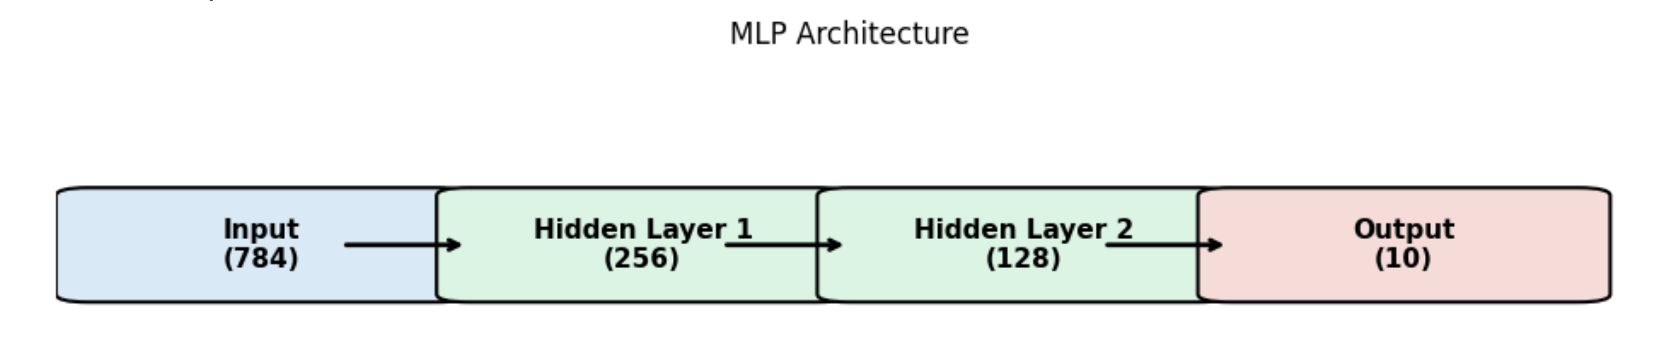
\includegraphics[width=0.85\textwidth]{mlp_architecture.png}
\caption{Architecture of the multilayer perceptron model.}
\label{fig:mlp_arch}
\end{figure}

\begin{figure}[H]
\centering
\includegraphics[width=0.85\textwidth]{mlp_curves.png}
\caption{Training and validation loss and accuracy curves for the MLP model.}
\label{fig:mlp_curves}
\end{figure}

\begin{figure}[H]
\centering
\includegraphics[width=0.75\textwidth]{mlp_confusion.png}
\caption{Confusion matrix of the MLP model.}
\label{fig:mlp_confusion}
\end{figure}

\subsection{MLP Results and Interpretation}

The MLP improved the baseline very clearly. In the final Kaggle notebook, it achieved \textbf{97.12\%} validation accuracy, a macro F1-score of \textbf{0.9710}, and a training time of \textbf{17.81 seconds} with \textbf{235,146} trainable parameters. The large improvement over the perceptron shows that hidden layers and nonlinear activation functions allow the model to learn more useful patterns.

\begin{figure}[H]
\centering
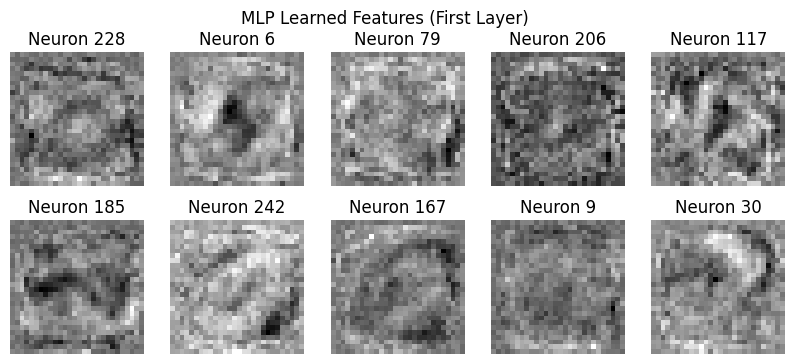
\includegraphics[width=0.80\textwidth]{mlp_features.png}
\caption{Learned first-layer features of the MLP model.}
\label{fig:mlp_features}
\end{figure}

The first-layer features in Figure~\ref{fig:mlp_features} are more abstract than the perceptron templates. They do not look like full digits. Instead, they capture parts of strokes and mixed pixel patterns. This shows that the MLP learns internal representations, not just one direct template for each class. Even so, it still works on flattened images, so it does not use image structure as naturally as a CNN.

\section{Convolutional Neural Networks}

\subsection{Why CNNs are Better Suited for Image Data}

An image is not just a long vector of numbers. It has spatial structure: neighboring pixels are related to one another, and important visual patterns such as edges, corners, and strokes are local. When an MLP flattens an image into a single vector, much of this spatial structure is ignored. A CNN is better suited for image data because it preserves and exploits this local organization.

\subsection{Convolution, Pooling, and Fully Connected Layers}

The core operation in a CNN is convolution. A small filter, or kernel, is moved across the image and computes a local weighted sum:
\begin{equation}
S(i,j) = (X * K)(i,j) = \sum_{m}\sum_{n} X(i+m,j+n)\,K(m,n)
\end{equation}
where $X$ is the input image (or feature map) and $K$ is the filter.

The output of a convolution layer is called a \textbf{feature map}. Each feature map highlights where a particular learned pattern appears in the input.

Pooling layers reduce spatial resolution and summarize nearby activations. For example, max-pooling selects the largest value in a local region:
\begin{equation}
P(i,j) = \max_{(u,v)\in \mathcal{R}_{ij}} S(u,v)
\end{equation}
where $\mathcal{R}_{ij}$ is a local pooling window.

After several convolution and pooling stages, the feature maps are flattened and passed to fully connected layers, which combine the learned features and perform the final classification.

\subsection{Key Ideas Behind CNNs}

CNNs are effective because of three key ideas:

\begin{itemize}
    \item \textbf{Local receptive fields:} each neuron in a convolution layer sees only a small region of the input. This is suitable for images because local patterns such as edges and strokes are meaningful building blocks.
    \item \textbf{Weight sharing:} the same filter is used across many spatial locations. This greatly reduces the number of parameters and allows the same pattern detector to work anywhere in the image.
    \item \textbf{Feature maps:} the outputs of convolution layers indicate where learned features occur, enabling the network to build progressively more complex representations.
\end{itemize}

These ideas make CNNs both more efficient and more appropriate for images than fully connected networks. A CNN does not need to relearn the same stroke detector at every pixel position; one shared filter can detect that stroke anywhere in the image.

\subsection{LeNet-Style Architecture}

LeNet is one of the earliest successful convolutional neural networks for handwritten character recognition. A standard LeNet-style design contains two convolutional stages, each followed by pooling, and then one or more fully connected layers. In the implementation used here, the first convolutional layer learns 6 filters and the second learns 16 filters before the representation is passed to a dense classifier.

\begin{figure}[H]
\centering
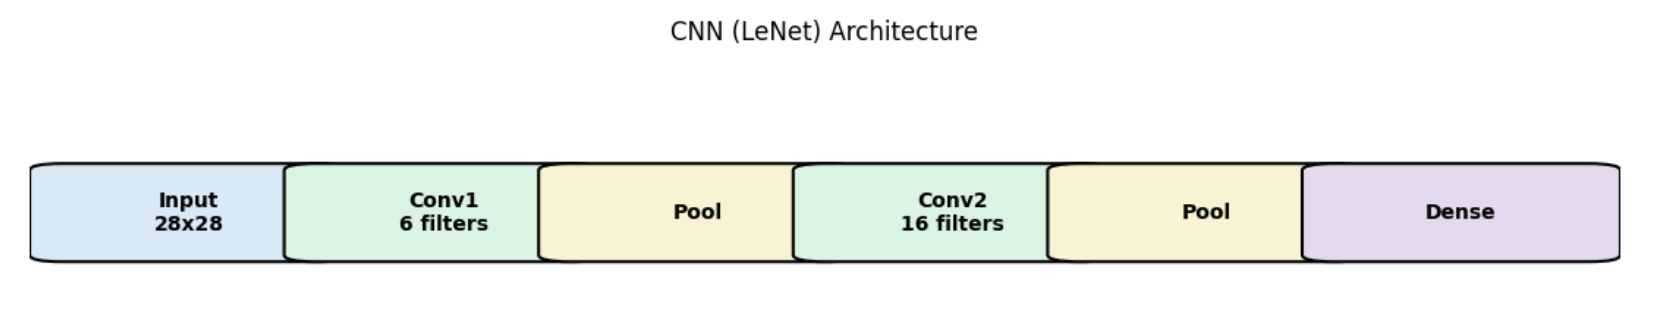
\includegraphics[width=0.85\textwidth]{cnn_architecture.png}
\caption{CNN (LeNet-style) architecture used for MNIST classification.}
\label{fig:cnn_arch}
\end{figure}

\subsection{Implementation Summary}

Unlike the perceptron and MLP, the CNN uses the original 2D image as input instead of flattening it at the start. The convolutional layers learn local patterns directly from the spatial layout of pixels. The pooling layers reduce resolution and improve robustness to small shifts, while the final fully connected layers combine the learned features and output probabilities over the 10 classes.

\begin{figure}[H]
\centering
\includegraphics[width=0.85\textwidth]{cnn_curves.png}
\caption{Training and validation loss and accuracy curves for the CNN model.}
\label{fig:cnn_curves}
\end{figure}

\begin{figure}[H]
\centering
\includegraphics[width=0.75\textwidth]{cnn_confusion.png}
\caption{Confusion matrix of the CNN model.}
\label{fig:cnn_confusion}
\end{figure}

\subsection{CNN Results and Interpretation}

The CNN gave the best overall result among the three models. In the final Kaggle notebook, it achieved \textbf{98.05\%} validation accuracy, a macro F1-score of \textbf{0.9803}, and a training time of \textbf{16.78 seconds} with \textbf{44,426} trainable parameters. Even though it uses far fewer parameters than the MLP, it performs better because it processes the image in a more suitable way.

\begin{figure}[H]
\centering
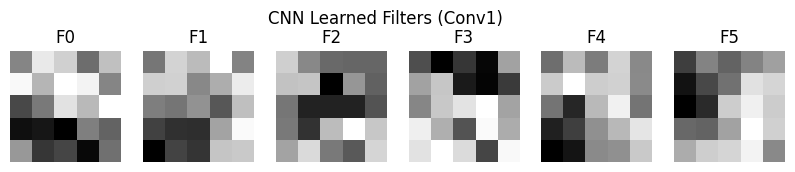
\includegraphics[width=0.82\textwidth]{cnn_filters.png}
\caption{Learned filters from the first convolutional layer of the CNN model.}
\label{fig:cnn_filters}
\end{figure}

The filters in Figure~\ref{fig:cnn_filters} act like simple pattern detectors. Some respond to vertical lines, some to curved strokes, and some to dark-to-light transitions. This is exactly what makes CNNs strong for image problems: they learn small local patterns first and then combine them into a full digit shape.

\section{Experimental Setup}

The three models were trained and evaluated on the MNIST handwritten digit dataset. A validation set was used during training so that both fitting and generalization could be monitored through loss curves and accuracy curves. The preprocessing and evaluation workflow can be summarized as follows:

\begin{itemize}
    \item input images were normalized so that pixel values lie in a stable numerical range,
    \item perceptron and MLP models used flattened 784-dimensional vectors as input,
    \item the CNN used the original 2D image structure,
    \item all models were trained for multiple epochs and monitored with validation metrics,
    \item performance was evaluated using accuracy, F1-score, training curves, confusion matrices, and training time.
\end{itemize}

The comparison is therefore fair in the sense that all three models solve the same classification problem on the same dataset, but they differ in representational power and in how they process the input.

\section{Results}

Table~\ref{tab:results} summarizes both the local validation results and the Kaggle public leaderboard scores. The ranking is the same in both evaluations: perceptron $<$ MLP $<$ CNN. This means the hidden Kaggle test set tells the same story as the local validation split.

\begin{table}[H]
\centering
\small
\setlength{\tabcolsep}{4pt}
\begin{tabular}{lccccc}
\toprule
\textbf{Model} & \textbf{Val Acc. (\%)} & \textbf{Val F1} & \textbf{Kaggle Score} & \textbf{Time (s)} & \textbf{Params} \\
\midrule
Perceptron & 91.76 & 0.9167 & 0.91800 & 11.90 & 7,850 \\
MLP & 97.12 & 0.9710 & 0.97503 & 17.81 & 235,146 \\
CNN (LeNet) & 98.05 & 0.9803 & 0.98539 & 16.78 & 44,426 \\
\bottomrule
\end{tabular}
\caption{Comparison of validation performance, Kaggle public scores, training time, and model size.}
\label{tab:results}
\end{table}

A few important observations are very easy to see:
\begin{itemize}
    \item The \textbf{perceptron} is the simplest model and gives the lowest score. It is useful as a starting point, but its linear nature limits performance.
    \item The \textbf{MLP} gives a large improvement. This shows that hidden layers and nonlinear activations really matter.
    \item The \textbf{CNN} gives the best validation accuracy and the best Kaggle score. This confirms that CNNs are the best fit for image classification in this assignment.
    \item The \textbf{CNN also uses far fewer parameters than the MLP} while still performing better. This highlights the efficiency of convolution and weight sharing.
\end{itemize}

\section{Detailed Performance Analysis}

\subsection{Effect of Depth}

Moving from the perceptron to the MLP increases the depth of the network. This leads to a large improvement in accuracy because the model no longer depends on a single linear separator. Instead, the hidden layers transform the input into intermediate representations that are easier to classify. This demonstrates that depth increases model capacity and allows the network to capture more complicated relationships between pixels and labels.

\subsection{Effect of Nonlinearity}

The addition of activation functions is essential. Without nonlinearity, the MLP would collapse into another linear model. ReLU and other nonlinear activations allow the network to create piecewise linear decision boundaries that better fit the structure of handwritten digits. The jump in performance from the perceptron to the MLP illustrates the practical importance of nonlinearity.

\subsection{Effect of Convolution}

The move from the MLP to the CNN introduces convolution. This does not simply add more parameters; rather, it changes how the model processes the data. By learning local filters and sharing them across the image, the CNN becomes more efficient and more suitable for the structure of image inputs. The improved results show that convolution is not just a deeper version of an MLP but a fundamentally better inductive bias for visual data.

\subsection{Interpretation of Training Curves}

The training and validation curves provide insight into the learning dynamics of each model. The perceptron converges quickly but plateaus early. The MLP continues improving because it has higher capacity, although this also makes overfitting more possible if regularization is weak. The CNN shows strong validation performance together with decreasing loss, indicating that it learns useful image features and generalizes well.

\subsection{Interpretation of Confusion Matrices}

The confusion matrices reveal which digit pairs are hardest to separate. Most errors occur between visually similar digits, such as digits with similar vertical strokes, loops, or curved endings. The perceptron shows the largest spread of mistakes because it cannot model subtle shape differences well. The MLP reduces many of these errors, while the CNN produces the cleanest confusion matrix because its learned features are better aligned with the structure of handwritten digits.

\section{Kaggle Competition Entries}

The assignment required at least one Kaggle entry for each classifier. This requirement was satisfied by creating three separate Kaggle notebooks and three separate CSV submission files. Keeping the models separate makes the comparison clean and easy to verify.

\begin{table}[H]
\centering
\small
\begin{tabular}{>{\raggedright\arraybackslash}p{2.2cm} >{\raggedright\arraybackslash}p{3.8cm} >{\raggedright\arraybackslash}p{4.1cm} c}
\toprule
\textbf{Model} & \textbf{Public notebook} & \textbf{Submission file} & \textbf{Public score} \\
\midrule
Perceptron & \href{https://www.kaggle.com/code/zaeemnasir7/perceptron-mnist}{Open} & \texttt{submission\_\allowbreak perceptron.csv} & 0.91800 \\
MLP & \href{https://www.kaggle.com/code/zaeemnasir7/mlp-mnist}{Open} & \texttt{submission\_\allowbreak mlp.csv} & 0.97503 \\
CNN (LeNet) & \href{https://www.kaggle.com/code/zaeemnasir7/cnn-lenet-mnist}{Open} & \texttt{submission\_\allowbreak cnn.csv} & 0.98539 \\
\bottomrule
\end{tabular}
\caption{Final Kaggle notebooks, submission files, and public leaderboard scores.}
\label{tab:kagglefiles}
\end{table}

\begin{figure}[H]
\centering
\includegraphics[width=0.96\textwidth]{kaggle_scores.png}
\caption{Screenshot of the Kaggle submissions page showing the three separate submission files and their public scores.}
\label{fig:kaggle}
\end{figure}

The Kaggle scores confirm the same pattern seen in local validation. The perceptron gives the lowest public score, the MLP performs much better, and the CNN achieves the best public leaderboard score of \textbf{0.98539}. This is strong evidence that the CNN generalizes best to unseen handwritten digits.

\section{Discussion}

The overall comparison becomes easy to understand when we ask a simple question: \emph{how much can each model learn from the image?} The perceptron can only create a linear decision rule, so it gives the weakest result. The MLP adds hidden layers and nonlinear activations, so it can learn more complex patterns and improves the score a lot. The CNN goes further by learning small image filters, which makes it the most natural model for handwritten digit images.

Another useful lesson is that more parameters do not automatically mean better performance. The MLP has many more parameters than the CNN, but the CNN still performs better. The reason is that the CNN uses a smarter design for image data: it learns local features and reuses them across the whole image.

The local validation results and the Kaggle leaderboard results tell the same story. This makes the final conclusion more reliable because the comparison is supported by both internal testing and external competition scoring.

\section{Conclusion}

This assignment showed, in a practical and easy-to-follow way, how model design affects classification performance on MNIST. All three models were able to learn the task, but they did not learn it equally well. The perceptron was the simplest baseline, the MLP improved the results by learning nonlinear patterns, and the CNN achieved the best overall performance because it is built for image data.

In very simple words, the final lesson is this: better models understand the image better. A linear model looks at the pixels in a basic way, an MLP learns richer combinations of pixels, and a CNN learns meaningful local patterns such as edges and strokes. That is why the CNN produced the best validation accuracy and the best Kaggle score.

The final Kaggle notebook links, separate submission files, leaderboard evidence, figures, and explanations are all included in this report, so the work is easy to verify and directly matches the assignment requirement.

\end{document}

